\section{Introduction}\label{sec:intro}
JavaScript is the de facto programming language in web development and,
moreover, blossoming beyond the web.
JavaScript has dominated client-side scripting of the web for over a decade.
JavaScript takes the unique position as the universal language operating in both
the browser and on a server in the form of Node.js.
The client-side frameworks such as React, Vue.js, and Angular have accelerated
the universal use of JavaScript.
The cross-platform frameworks like React Native and Electron have spread
JavaScript to the new domains like mobile and desktop beyond the web.
This is only possible thanks to JavaScript's easy operation in development and
deployment with scripting language characteristics such as dynamic and
interpreted language features~\cite{weaklySPE}.


However, such features make it difficult to support developer tools that require
statically reasoning about semantics of JavaScript programs such as call graph
construction, type checking, optimization, and bug detection.
For example, the combination of the JavaScript features: dynamically-computed
property name, prototype chain, and first-class function, makes call graph
construction extremely challenging.
Even a minor precision loss at property name can cause reading all methods in
the object and its prototype chain, including hundreds of built-ins, that
results in useless analysis results.
In static analyses of Java, the benchmark results clearly show the trade-off
between precision and performance~\cite{introspective, data-driven}, a low
degree of context sensitivity shows a high performance but low precision.
In the case of JavaScript, the relationship between precision and performance is
more complex due to the spurious callee explosion.
Low precision tends to cause the large number of spurious callees that
significantly degrades the performance~\cite{correlation, determinacy-jQuery, weaklySPE, value-refinement}.


For this reason, recent studies on JavaScript static analysis have developed
to improve analysis precision against this challenge.
Madsen et al.~\cite{string, regex, combining-string} presented sophisticated
abstract domains for strings.
Park et al. proposed higher degrees of context sensitivity for loops~\cite{lsaECOOP, lsaSPE}.
Relations between object properties have aided to analysis precision~\cite{correlation, weaklyAPLAS, weaklySPE}.
The idea stretches from property name to non-local variables and types for
predicate functions~\cite{value-partitioning}.
The on-demand backward analyses~\cite{value-refinement} refines imprecise values
for property writes.


Unfortunately, computation cost of high degrees of sensitivity remains as it is
but the snowball cost of low precision is much larger than that.
So it is difficult to scale up JavaScript static analysis even though we give up
analysis precision.
We address the scalability issue of high degrees of sensitivity through a
combined approach of static and dynamic analyses.


Existing combined approaches derive three kinds of benefits by dynamic analysis.
Dynamic analyses~\cite{jalangi, dlint} can run on a highly-optimized
JavaScript engine like V8, so it can boost up analysis performance.
There is no precision loss coming from limitations of abstract domains and
sensitivities if the dynamic analysis terminates~\cite{determinacy, concerto}.
Note that in this case of combined analyses does not sacrifice soundness.
Dynamic analysis can pass by opaque codes that require extra handling for static
analysis~\cite{battles, sra}.


However, the existing combined analyses are limited to maximize benefits of
dynamic analysis.
Staged analyses first collect particular information by dynamic analysis and
augment static analysis with the information~\cite{blendedJava, eha}.
Dynamic information can be determinacy facts~\cite{determinacy}, call graphs~\cite{tunable}
object creations~\cite{blendedJS}, or entire heaps at specific program points~\cite{battles}.
Once static analysis starts, staged analyses does not utilize more dynamic information.
The other design of combined analysis divides a whole program into two parts~\cite{concerto}.
One (framework code) for the dynamic analysis  and the other (user code) for the
static analysis.
The policy to divde a program is predefined and syntactic, so never changes
during analysis.


We present a more flexible and fine-grained method to combine two analyses to
maximize the benefits.
Our idea enables abstract interpretation to use the dynamic analysis on demand
to speed up the analysis while preserving soundness, so we call that adding
dynamic shortcuts.
We extend a dynamic analysis to work as long as possible despite of the presence
of abstract values by laziness.
The analysis goes on the concrete engine as much as possible until it meets
operations with non-deterministic values by abstract values or analysis
sensitivity that the concrete engine cannot handle.
When the dynamic shortcut meets non-determinism, the analysis switches to
the traditional static analysis and uses its abstract semantics to handle that.
As soon as analysis sensitivity is deterministic, it continues to take the
dynamic shortcut again.

\begin{figure}
  \centering
  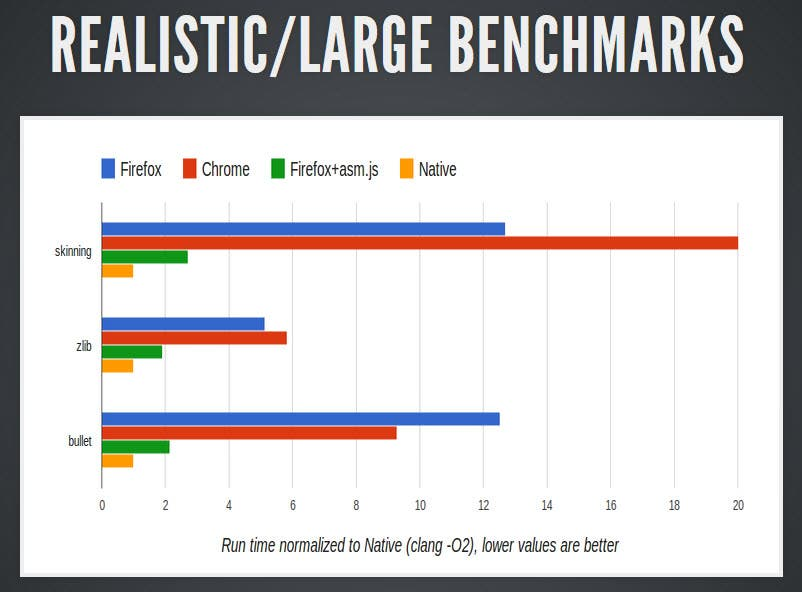
\includegraphics[width=\linewidth]{benchmark_performance}
  \caption{The performances of static and dynamic analyses on deterministic benchmarks}
  \label{fig:performance}
\end{figure}

Our key observation is that high degrees of sensitivity increase the use of
concrete semantics during analysis and utilizing an optimzied engine like V8 is
the fast way to apply concrete semantics.
\inred{As shown in Figure~\ref{fig:performance}. dynamic analyses on V8 engine show
25x fatster on average than the fastest static analyzer.}
Our design is not limited to any predefined features including program point and
does not harmful to the soundness of the original static analysis.


%We have demonstrated how dynamic shortcut maximize benefits of dynamic analysis.
%We have implemetned our method by extending the existing JavaScript static
%analyzer.
%We found that using dynamic shortcut significantly increased performance for
%benchmark programs enhanced with abstracted input.

In summary, the contributions of this paper are as follows.
\begin{itemize}
\item We formally describe the high-level idea of adding dynamic shortcuts, a
  technique for combining static and dynamic analyses into fine-grained level on
  the general abstract interpretation framework.
\item We actualize our method by extending the existing JavaScript static analyzer SAFE 2.0.
\item We empirically evaluate our technique using the implementation.
  We find that using dynamic shortcut significantly increased performance for
  benchmark programs enhanced with abstracted input that existing combined
  analysis designs cannot handle.
\end{itemize}
The remainder of this paper is organized as follows.
In Section~\ref{sec:motivation}, we explain more details about limitations of
existing techniques and our solution with the real-world JavaScript programs.
Section~\ref{sec:formal} formalizes adding dynamic shortucts on abstract
interpretation.
We explain JavaScript related features formalized with core language of
JavaScript in Section~\ref{sec:javascript}.
Section~\ref{sec:implementation} describes key implementation techniques like the synchronizetion of two analyses.
We evaluate our idea using real-world benchmarks in Section~\ref{sec:eval}.
We organize related work in Section~\ref{sec:related}, and we conclude in Section~\ref{sec:conclusion}.

%There are almost 200 million active websites out of over 1.8 billion sites on the entire web.
%https://www.internetlivestats.com/total-number-of-websites/
%JavaScript is used as client-side programming language by 96.9\% of all the websites.
%https://w3techs.com/technologies/history_overview/client_side_language/all/y
